\documentclass{beamer}

\usepackage{préambule}

\begin{document}

\begin{frame}
	\begin{center}
		\LARGE
		\uline{Le problème du billard}
	\end{center}

	On considère un billard rectangulaire, quadrillé de manière régulière.

	On envoie une bille depuis l'un des sommets du billard, et celle-ci rebondit jusqu'à ce qu'elle ressorte à l'un des quatres sommets du billard.

	\begin{center}
		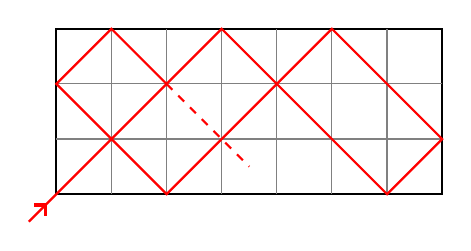
\begin{tikzpicture}[scale=0.7]
			\newcommand{\billardX}{7}
			\newcommand{\billardY}{3}
			\draw[thick] (0,0) -- ++(\billardX,0) -- ++(0,\billardY) -- ++(-\billardX,0) -- cycle;
			\foreach \x in {1,...,6} {
					\draw[thin,gray] (\x,0) -- ++(0,\billardY);
				}
			\foreach \y in {1,...,2} {
					\draw[thin,gray] (0,\y) -- ++(\billardX,0);
				}
			\draw[red,thick] (-0.5,-0.5) -- (0,0) -- ++(3,3) -- ++(3,-3) -- ++(1,1) -- ++(-2,2) -- ++(-3,-3) -- ++(-2,2) -- ++(1,1) -- ++(1,-1);
			\draw[red,thick,dashed] (2,2) -- ++(1.5,-1.5);
			\draw[red,very thick] (-0.4,-0.2) -- (-0.2,-0.2) -- (-0.2,-0.4);
		\end{tikzpicture}
	\end{center}

	Peut-on déterminer à l'avance le nombre de carreaux traversés par la bille en fonction des dimensions du billard ?
\end{frame}

\end{document}